%% img/LPadComplexity.tex
%% Copyright 2019 Andrea Berlingieri
%
% This work may be distributed and/or modified under the
% conditions of the LaTeX Project Public License, either version 1.3
% of this license or (at your option) any later version.
% The latest version of this license is in
%   http://www.latex-project.org/lppl.txt
% and version 1.3 or later is part of all distributions of LaTeX
% version 2005/12/01 or later.
%
% This work has the LPPL maintenance status `maintained'.
%
% The Current Maintainer of this work is Andrea Berlingieri.
%
% This work consists of all files listed in manifest.txt
\documentclass{standalone}

\usepackage{TikzStyle}
\usepackage{mystyle}

\newcommand{\gpoint}[2]{%
\filldraw [gray] (#1,#2) circle [radius=2pt]
}

\begin{document}
    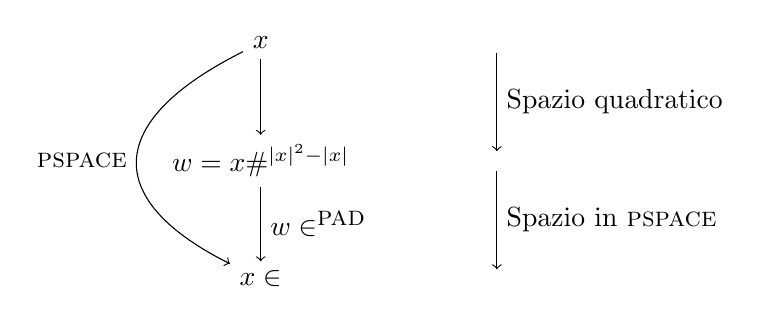
\begin{tikzpicture}
        \node (x) at (0,0) {$x$};
        \node (xp) at (0,-1.5) {$w = x\#^{|x|^{2}-|x|}$};
        \node (xinL) at (0,-3) {$x \in \Lang$};
        \draw[->] (x) -- (xp);
        \draw[->] (xp) -- (xinL) node [pos=0.5, right] {$w \in \Lang^{\textsc{pad}}$};
        \node (c1) at (3,0) {};
        \node (c2) at (3,-1.5) {};
        \node (c3) at (3,-3) {};
        \draw[->] (c1) -- (c2) node [pos=0.5,right] {Spazio quadratico};
        \draw[->] (c2) -- (c3) node [pos=0.5,right] {Spazio in $\textsc{pspace}$};
        \draw[->] (x) .. controls (-2,-1) and (-2,-2) .. (xinL) node [pos=0.5,left]
        {$\textsc{pspace}$};
    \end{tikzpicture}
\end{document}
